\documentclass[answers]{exam}
\usepackage{texPreamble}
\usepackage{relsize}
\usepackage{tabularx}
\extraheadheight{0.25in}
\extrafootheight{1.0in}
\extrawidth{1in}
% ----------------------------------------------------------------

\begin{document}
%\relscale{1.4}
    \section{JIT 5.4: Graphs involving $\sin x$ and $\cos x$}
    \begin{center}
      \begin{tikzpicture}[scale=1.0]
        \begin{groupplot}[
          group style={group size=1 by 2, vertical sep=1cm},
          axis lines=center,
          axis line style={->},
          xmin=-7, xmax=7,
          ymin=-1.25, ymax=1.25,
          xtick={-6.28318, -4.7123889, ..., 6.28318},
          xticklabels={$-2\pi$, $-\frac{3\pi}{2}$,$-\pi$, $-\frac{\pi}{2}$, ,
             $\frac{\pi}{2}$,$\pi$, $\frac{3\pi}{2}$, $2\pi$},
          height=1.1in, width=0.95\linewidth,
          ticklabel style={font=\small, inner sep=0.75, fill=white},
          every axis plot/.append style={line width=0.95pt},
          ]
        \nextgroupplot[xlabel=$\cos(\theta)$, xlabel style={at={(ticklabel* cs:1)},anchor=north west}]
          \addplot[domain=-6.28:6.28, blue, samples=101] {cos(deg(x))};
        \nextgroupplot[xlabel=$\sin(\theta)$, xlabel style={at={(ticklabel* cs:1)},anchor=north west}]
          \addplot[domain=-6.28:6.28, blue, samples=101] {sin(deg(x))};
        \end{groupplot}
      \end{tikzpicture}
    \end{center}
    
    \vspace*{\stretch{1}}
    \begin{ex*}
      On $\sbrkt{0,2\pi}$, graph $\sin x$, $1+ \sin x$ and $\sin\parens{x-\dfrac{\pi}{2}}$.
      \begin{center}
        \begin{tikzpicture}
          \begin{groupplot}[
              group style={group size=1 by 2, vertical sep=50pt},
              axis lines=center,
              axis line style={->},
              xmin=0, xmax=7,
              ymin=-1.25, ymax=2.5,
              xtick={-6.28318, -4.7123889, ..., 6.28318},
              xticklabels={$-2\pi$, $-\frac{3\pi}{2}$,$-\pi$, $-\frac{\pi}{2}$, ,
                 $\frac{\pi}{2}$,$\pi$, $\frac{3\pi}{2}$, $2\pi$},
              height=2in, width=0.95\linewidth,
              ticklabel style={font=\small, inner sep=0.75, fill=white},
              every axis plot/.append style={line width=0.95pt},
              legend style={at={(axis cs:7*3.14/4,-1.25)},anchor=north west},
              ]
            \nextgroupplot[ymin=-1.25, ymax=2.5]
              \addplot[domain=0:6.28, blue, samples=101, dashed] {sin(deg(x))};
              \addlegendentry{$\sin(x)$};
              \addplot[domain=0:6.28, blue, samples=101] {1+sin(deg(x))};
              \addlegendentry{$1+\sin(x)$};
            \nextgroupplot[ymin=-1.25, ymax=1.5, height=1.95in]
              \addplot[domain=0:6.28, blue, samples=101, dashed] {sin(deg(x))};
              \addlegendentry{$\sin(x)$};
              \addplot[domain=0:6.28, blue, samples=101] {sin(deg(x-3.14/2))};
              \addlegendentry{$\sin(x-\frac{\pi}{2})$};
              \draw[->, line width = 0.95pt] (axis cs: 3.14/6, 0.5) -- (axis cs: 2*3.14/3-0.075, 0.5);
              \draw[->, line width = 0.95pt] (axis cs: 7*3.14/6, -0.5) -- (axis cs: 5*3.14/3-0.075, -0.5);
          \end{groupplot}
        \end{tikzpicture}
      \end{center}
    \end{ex*}
    \begin{defn*}
      A shift to the left or right of a wave shaped graph, such as $\sin x$ or $\cos x$, is called a \textbf{phase shift}.
    \end{defn*}
    \vspace*{\stretch{1}}
    \pagebreak

    \begin{ex*}
      Vertical scaling:
      \begin{center}
        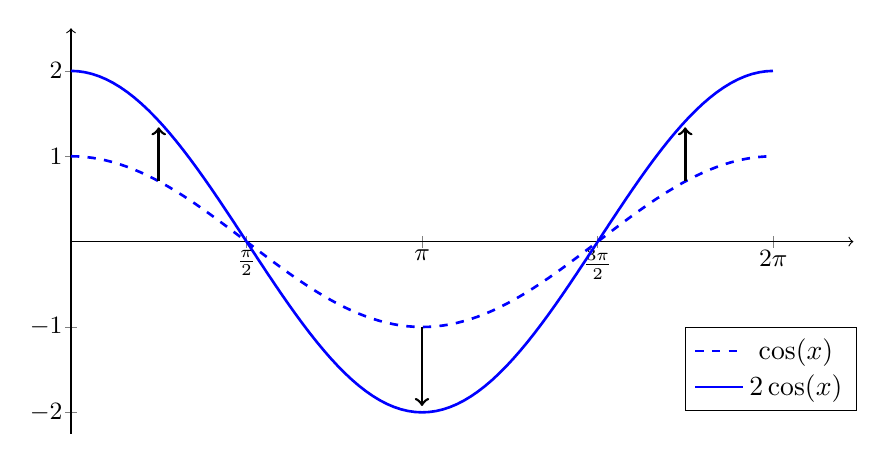
\begin{tikzpicture}
          \begin{axis}[
              axis lines=center,
              axis line style={->},
              xmin=0, xmax=7,
              ymin=-2.25, ymax=2.5,
              xtick={-6.28318, -4.7123889, ..., 6.28318},
              xticklabels={$-2\pi$, $-\frac{3\pi}{2}$,$-\pi$, $-\frac{\pi}{2}$, ,
                 $\frac{\pi}{2}$,$\pi$, $\frac{3\pi}{2}$, $2\pi$},
              ytick={-2,-1,1,2},
              height=2.65in, width=0.95\linewidth,
              ticklabel style={font=\small, inner sep=0.75, fill=white},
              legend style={at={(axis cs:7*3.14/4,-1)},anchor=north west},
              every axis plot/.append style={line width=0.95pt},
              ]
            \addplot[domain=0:6.28, blue, samples=101, dashed] {cos(deg(x))};
            \addlegendentry{$\cos(x)$};
            \addplot[domain=0:6.28, blue, samples=101] {2*cos(deg(x))};
            \addlegendentry{$2\cos(x)$};
            \draw[->, line width = 0.95pt] (axis cs: 3.14, -1) -- (axis cs: 3.14, -2+0.075);
            \draw[->, line width = 0.95pt] (axis cs: 3.14/4, 0.707) -- (axis cs: 3.14/4, 1.414-0.075);
            \draw[->, line width = 0.95pt] (axis cs: 7*3.14/4, 0.707) -- (axis cs: 7*3.14/4, 1.414-0.075);
          \end{axis}
        \end{tikzpicture}
      \end{center}
    \end{ex*}

      \begin{defn*}
        The \textbf{amplitude} of a sinusoidal graph is equal to \sfrac12 of the distance from the top to the bottom of the waves.
      \end{defn*}
      \begin{center}
        \begin{tikzpicture}
          \begin{groupplot}[
              group style={group size=1 by 2, vertical sep=55pt},
              axis lines=center,
              axis line style={->},
              xmin=0, xmax=7,
              ymin=-1.25, ymax=1.5,
              xtick={-6.28318, -4.7123889, ..., 6.28318},
              xticklabels={$-2\pi$, $-\frac{3\pi}{2}$,$-\pi$, $-\frac{\pi}{2}$, ,
                 $\frac{\pi}{2}$,$\pi$, $\frac{3\pi}{2}$, $2\pi$},
              height=2in, width=0.95\linewidth,
              ticklabel style={font=\small, inner sep=0.75, fill=white},
              legend style={at={(axis cs:7*3.14/4,-1.25)},anchor=north west},
              every axis plot/.append style={line width=0.95pt},
              ]
            \nextgroupplot
              \addplot[domain=0:6.28, blue, samples=101, dashed] {cos(deg(x))};
              \addlegendentry{$\cos(x)$};
              \addplot[domain=0:6.28, blue, samples=101] {-cos(deg(x))};
              \addlegendentry{$-\cos(x)$};
              \draw[->, line width = 0.95pt] (axis cs: 3.14, -1) -- (axis cs: 3.14, 1-0.075);
              \draw[->, line width = 0.95pt] (axis cs: 3.14/4, 0.707) -- (axis cs: 3.14/4, -0.707+0.075);
              \draw[->, line width = 0.95pt] (axis cs: 7*3.14/4, 0.707) -- (axis cs: 7*3.14/4, -0.707+0.075);
            \nextgroupplot
              \addplot[domain=0:6.28, blue, samples=101, dashed] {cos(deg(x))};
              \addlegendentry{$\cos(x)$};
              \addplot[domain=0:6.28, blue, samples=101] {0.5*cos(deg(x))};
              \addlegendentry{$\sfrac{1}{2}\cos(x)$};
              \draw[->, line width = 0.95pt] (axis cs: 3.14, -1) -- (axis cs: 3.14, -0.5-0.05);
              \draw[->, line width = 0.95pt] (axis cs: 3.14/4, 0.707) -- (axis cs: 3.14/4, 0.707/2+0.05);
              \draw[->, line width = 0.95pt] (axis cs: 7*3.14/4, 0.707) -- (axis cs: 7*3.14/4, 0.707/2+0.05);
          \end{groupplot}
        \end{tikzpicture}
      \end{center}
      \vspace*{\stretch{1}}
      \pagebreak
        
      \begin{defn*}
        \begin{itemize}
          \item The \textbf{period} of the oscillating function is the length of a cycle.
          \item For functions of the form $\sin(a x)$ the \textbf{period} is given by $\omega=\frac{2\pi}{a}$. The same holds for $\cos(a x), \sec(ax)$ and $\csc(ax)$ since these 4 functions all have a \textbf{period} of $2\pi$.
          \item When using $\tan(ax), \cot(ax)$  we need to divide $a$ by the functions original period: $\pi \Rightarrow$ \textbf{period} is $\omega=\dfrac{\pi}{a}$.
        \end{itemize}
      \end{defn*}

    \begin{center}
      \begin{tikzpicture}
        \begin{groupplot}[
            group style={group size=1 by 2, vertical sep=2cm},
            axis lines=center,
            axis line style={->},
            xmin=0, xmax=6.5,
            ymin=-1.25, ymax=1.5,
            xtick={-6.28318, -4.7123889, ..., 6.28318},
            xticklabels={$-2\pi$, $-\frac{3\pi}{2}$,$-\pi$, $-\frac{\pi}{2}$, ,
               $\frac{\pi}{2}$,$\pi$, $\frac{3\pi}{2}$, $2\pi$},
            height=2in, width=0.95\linewidth,
            ticklabel style={font=\small, inner sep=0.75, fill=white},
            legend style={at={(axis cs:7*3.14/4,-1.3)},anchor=north west},
            every axis plot/.append style={line width=0.95pt},
            ]
          \nextgroupplot
            \addplot[domain=0:6.28, blue, samples=101, dashed] {sin(deg(x))};
            \addlegendentry{$\sin(x)$};
            \addplot[domain=0:3.14, blue, samples=101] {sin(deg(2*x))};
            \addlegendentry{$\sin(2x)$};
            \draw[dashed, line width =0.95] (3.14,-1.25) -- (3.14,1.5);
            \draw[->, line width =0.95] (0,1.25) -- (3.14,1.25) node[below, pos=0.85] {$\omega=\pi$};
          \nextgroupplot[
            xmax=13, xtick={-6.28318, -4.7123889, ..., 12.566},
            xticklabels={$-2\pi$, $-\frac{3\pi}{2}$,$-\pi$, $-\frac{\pi}{2}$, ,
               $\frac{\pi}{2}$,$\pi$, $\frac{3\pi}{2}$, $2\pi$, $\frac{5\pi}{2}$,
               $3\pi$, $\frac{7\pi}{2}$, $4\pi$},
            legend style={at={(axis cs:7*3.14/2,-1.3)},anchor=north west},]
            \addplot[domain=0:6.28, blue, samples=101, dashed] {sin(deg(x))};
            \addlegendentry{$\sin(x)$};
            \addplot[domain=0:12.566, blue, samples=101] {sin(deg(0.5*x))};
            \addlegendentry{$\sin\parens{\sfrac{x}{2}}$};
            \draw[dashed, line width =0.95] (4*3.14,-1.25) -- (4*3.14,1.5);
            \draw[->, line width =0.95] (0,1.25) -- (4*3.14,1.25) node[below, pos=0.9] {$\omega=4\pi$};
        \end{groupplot}
      \end{tikzpicture}
    \end{center}
    \begin{defn*}
      The \textbf{frequency} is given by $f=\dfrac{1}{\omega}$.
    \end{defn*}
    \vspace*{\stretch{1}}
    
    \pagebreak
\end{document}